\bookchapter{บทที่ 60: ตั้งสภาพแวดล้อมการพัฒนา — Xcode กับโปรเจกต์แรก}

\chapterintro{จะทำงานให้เป็น ต้องลับเครื่องมือให้คมก่อน บทนี้เราจะสร้าง “ห้องครัว” ให้พร้อม: ติดตั้ง Xcode ให้ซิมูเลเตอร์รันผ่าน สร้างโปรเจกต์ iOS แรกในชีวิต แล้วแกะโครงสร้างโปรเจกต์ให้เห็นชัด ๆ พอเครื่องพร้อม คุณจะได้เห็นเป็นครั้งแรกว่าโค้ดที่เขียนกลายเป็นปุ่มที่กดได้จริง ๆ — วินาทีนี้ หลายคนจำได้ตลอดชีวิต}

\booksection{เตรียม Mac สักเครื่อง}

เริ่มจากข้อกีดขวางก่อน: การพัฒนา iOS ต้องทำบน macOS เท่านั้น ถ้ายังไม่มี Mac มีทางเลือกสามทาง: ซื้อสักเครื่อง (แม้แต่ Mac mini หรือ MacBook Air มือสองก็ใช้ได้), เช่า Mac บนคลาวด์ระยะสั้น, หรือไปอ่านภาคที่ 8 “ลงมือพัฒนา Android” (ใช้ Windows ก็ทำได้) ก่อน

\begin{center}
\begin{tabularx}{\linewidth}{|X|X|X|}
\hline
\textbf{รายการตั้งค่า} & \textbf{ค่าขั้นต่ำ} & \textbf{ระดับสบาย (แนะนำ)} \tabularnewline
\hline
ชิป & Apple Silicon (M1 ขึ้นไป) & M2 หรือใหม่กว่า \tabularnewline
หน่วยความจำ & 8GB & 16GB \tabularnewline
ดิสก์ & สำรองพื้นที่ 40GB+ (ตัว Xcode กินพื้นที่เยอะ) & เริ่มต้นที่ 256GB \tabularnewline
ระบบปฏิบัติการ & macOS เวอร์ชันล่าสุด & เปิดอัปเดตอัตโนมัติไว้ \tabularnewline
\hline
\end{tabularx}
\end{center}

\begin{center}\small\color{gray}สเปกอ้างอิงเครื่อง Mac สำหรับพัฒนา (สิงหาคม 2026)\end{center}

\begin{tcbinfo}{เคล็ดลับ: ไม่มี Mac ก็เริ่มเรียนภาษาได้ก่อน}
Swift Playgrounds ที่ฟรีบน iPad เรียนพื้นฐานภาษา Swift ได้ (ไม่ต้องมี Mac); แม้แต่บน iPhone ก็ติดตั้งได้ ลองเล่นความรู้ภาษาจากบทที่ 61 ใน Playgrounds ให้คล่องก่อน พอได้ Mac มาครองก็ออกตัวได้ทันที “ลับเคียวไม่เสียเวลาตัดฟืน” พูดถึงเรื่องนี้แหละ

\end{tcbinfo}

\booksection{ติดตั้ง Xcode}

Xcode คือ IDE ทางการของ Apple ใช้ฟรี ติดตั้งเสร็จในสามขั้นตอน:

\begin{enumerate}
  \item เปิด App Store บน Mac ค้นหา "Xcode" แล้วกดติดตั้ง — ระวังว่ามันมีหลาย GB หาช่วงเน็ตชิล ๆ ทำ;
  \item พอติดตั้งเสร็จแล้วเปิดครั้งแรก ยอมรับข้อตกลง ติดตั้งคอมโพเนนต์ให้ครบ (ทำเองอัตโนมัติ);
  \item เมนู Xcode Settings Locations ยืนยันว่า Command Line Tools ถูกเลือกไว้แล้ว — เครื่องมือบรรทัดคำสั่งเป็นเงื่อนไขของสคริปต์และเครื่องมือภายนอกจำนวนมาก.
\end{enumerate}

\begin{tcbwarn}{ข้อควรรู้: เกมจับคู่เวอร์ชัน Xcode กับระบบ}
Xcode รุ่นใหม่มักต้องการ macOS ล่าสุด ส่วน Mac เครื่องเก่าจะติดค้างที่เวอร์ชันเก่า ตอนขึ้น App Store Apple จะให้ใช้ Xcode ที่ใหม่พอสมควรบิลด์ (มักมีช่วงผ่อนปรนให้) ดังนั้นอย่าผลัดการอัปเดตระบบนานเกินไป — นักพัฒนา iOS คือกลุ่มที่ “วิ่งไล่เวอร์ชันใหม่” ขยันที่สุดกลุ่มหนึ่ง

\end{tcbwarn}

\booksection{สร้างโปรเจกต์แรกของคุณ}

เปิด Xcode Create New Project เลือก iOS เทมเพลต App แล้วกรอก:

\begin{center}
\begin{tabularx}{\linewidth}{|X|X|X|}
\hline
\textbf{รายการตั้งค่า} & \textbf{กรอกอะไร} & \textbf{คำอธิบาย} \tabularnewline
\hline
Product Name & MyFirstApp & ชื่อแอป \tabularnewline
Team & Apple ID ของคุณ (ฟรี) & ใช้สำหรับเซ็น บัญชีส่วนตัวก็พอ \tabularnewline
Organization Identifier & com.example & รวมกับ Product Name เป็นตัวระบุแพ็กเกจ \tabularnewline
Interface & SwiftUI & เฟรมเวิร์กเส้นหลักของหนังสือเล่มนี้ \tabularnewline
Language & Swift & ไม่ต้องอธิบาย \tabularnewline
\hline
\end{tabularx}
\end{center}

\begin{center}\small\color{gray}5 อย่างที่ต้องกรอกตอนสร้างโปรเจกต์\end{center}

กด Create แล้ว Xcode จะสร้างโปรเจกต์ที่รันได้ทันทีขึ้นมา มุมซ้ายบนเลือกซิมูเลเตอร์สักเครื่อง (เช่น iPhone 17) กด > รัน — ไม่กี่วินาทีต่อมา บนจอซิมูเลเตอร์จะมีหน้าต่างเขียนว่า “Hello, world!” แอป iOS ตัวแรกของคุณถือกำเนิดแล้ว

\booksection{แกะโครงสร้างโปรเจกต์: ไฟล์แต่ละตัวทำอะไร}

ด้านซ้ายคือตัวนำทางโปรเจกต์ มือใหม่แค่ต้องรู้จักไม่กี่ตัวนี้:

\begin{center}
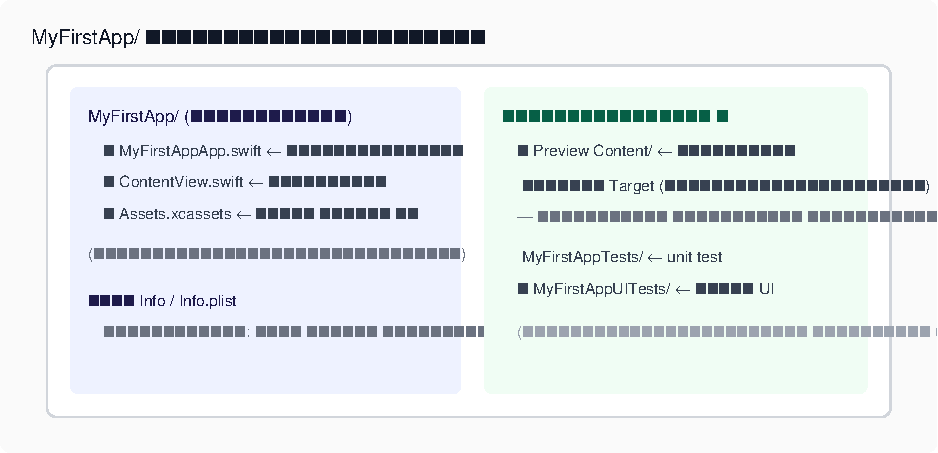
\includegraphics[width=0.92\linewidth]{figures/fig-di-liu-shi-zhang-1}
\\[2pt]\small ภาพที่ 2: โครงสร้างโปรเจกต์ Xcode ที่มือใหม่ต้องรู้
\end{center}

\begin{itemize}
  \item MyFirstAppApp.swift: จุดเริ่มของโปรแกรม ใน SwiftUI มันมีแค่ไม่กี่บรรทัด — “สตาร์ท แล้วแสดงหน้าหลัก”;
  \item ContentView.swift: วิวหน้าจอหลัก ทุกอย่างที่คุณเห็นตอนนี้อยู่ในไฟล์นี้;
  \item Assets.xcassets: คลังทรัพยากร — ไอคอน รูปภาพ สี เก็บไว้ที่นี่;
  \item การตั้งค่า Target: กดไอคอนโปรเจกต์สีน้ำเงินด้านซ้ายเข้าไป เลขเวอร์ชัน iOS ขั้นต่ำ และการเซ็น อยู่ในนี้หมด ชื่อที่แสดงของแอปกับไอคอนก็ตั้งที่นี่เช่นกัน.
\end{itemize}

\booksection{ดีบักบนเครื่องจริง: ติดตั้งแอปลง iPhone ของคุณ}

\booksection{เทคนิคทำงานไวใน Xcode: “โกงเกม” 5 ปุ่มลัดของมือใหม่}

ใช้พวกนี้จนคล่อง คุณจะดู “เป็นมืออาชีพ” ขึ้นทันที:

\begin{center}
\begin{tabularx}{\linewidth}{|X|X|X|}
\hline
\textbf{การกระทำ} & \textbf{ปุ่มลัด} & \textbf{หน้าที่} \tabularnewline
\hline
รัน & CmdR & คอมไพล์แล้วรันขึ้นมา \tabularnewline
เปิด/สลับพรีวิวแคนวาส & OptionCmd & สวิตช์เปิดพรีวิวแบบเห็นตามที่เขียน \tabularnewline
จัดย่อหน้าให้เรียบร้อย & CtrlI & จัดย่อหน้าของโค้ดที่เลือกให้อัตโนมัติ \tabularnewline
เปิดไฟล์อย่างรวดเร็ว & CmdO & พิมพ์ชื่อไฟล์แล้วเปิดทันที (ใช้บ่อยที่สุด!) \tabularnewline
คอมเมนต์/เลิกคอมเมนต์ & Cmd/ & เปิด-ปิดโค้ดส่วนไหนก็ได้ระหว่างดีบัก \tabularnewline
\hline
\end{tabularx}
\end{center}

\begin{center}\small\color{gray}ปุ่มลัดใช้บ่อยของ Xcode (ชุดห้าสำหรับมือใหม่)\end{center}

โบนัสซ่อนอยู่อีกสองอย่าง: เปิดซิมูเลเตอร์หลายตัวพร้อมกัน (รัน iPhone กับ iPad เทียบเลย์เอาต์ได้ในเวลาเดียว) และคลังโค้ดสั้น (ลากโค้ดที่ใช้บ่อยไปวางในแผง Snippets ด้านขวา คราวหน้าแทรกได้ด้วยคลิกเดียว) — เครื่องมือเพิ่มประสิทธิภาพใช้ก่อนเลย มือมันจะคล่องเอง

\booksection{ดีบักบนเครื่องจริง: ติดตั้งแอปลง iPhone ของคุณ}

ซิมูเลเตอร์ดีอยู่หรอก แต่ปลายทางคือเครื่องจริง ใช้ Apple ID ฟรีก็ดีบักบนเครื่องจริงได้:

\begin{enumerate}
  \item ต่อสายข้อมูลกับ iPhone (หรือดีบักไร้สายผ่าน Wi-Fi เดียวกัน);
  \item ในรายการอุปกรณ์ด้านบนของ Xcode เลือกเครื่องของคุณ ครั้งแรกจะมีข้อความให้ล็อกอิน Apple ID และตั้งค่าการเซ็นให้อัตโนมัติ;
  \item บน iPhone ไปที่ [การตั้งค่า] [ทั่วไป] [VPN และการจัดการอุปกรณ์] เชื่อถือใบรับรองนักพัฒนาของคุณ;
  \item กด > แอปจะถูกติดตั้งลงเครื่องจริง.
\end{enumerate}

\begin{tcbwarn}{ข้อควรรู้: “ข้อจำกัด 7 วัน” ของบัญชีฟรี}
แอปที่เซ็นด้วย Apple ID ฟรีจะหมดอายุใน 7 วัน (รันใหม่อีกครั้งก็ต่ออายุได้) นี่คือกลไกกันการใช้ในทางที่ผิดของ Apple ช่วงเรียนรู้ใช้ได้สบาย; บัญชีนักพัฒนาแบบเสียเงิน (99 ดอลลาร์/ปี) ไม่มีข้อจำกัดนี้ รายละเอียดอยู่ในบทที่ 67

\end{tcbwarn}

\booksection{ลองมือจริง + หนังสือฉุกเฉินเมื่อเจอ error ที่พบบ่อย}

\booksection{ลองมือจริง + หนังสือฉุกเฉินเมื่อเจอ error ที่พบบ่อย}

เปิด ContentView.swift เปลี่ยนข้อความใน Text(“Hello, world!”) เป็นชื่อของคุณ กด CmdR รันใหม่ — ไม่กี่วินาทีต่อมาชื่อคุณก็โผล่บนซิมูเลเตอร์ ยินดีด้วย คุณครบวงจร “แก้โค้ด คอมไพล์ ติดตั้ง รัน” ครั้งแรกแล้ว

\begin{center}
\begin{tabularx}{\linewidth}{|X|X|X|}
\hline
\textbf{อาการ error} & \textbf{สาเหตุที่พบบ่อย} & \textbf{วิธีแก้} \tabularnewline
\hline
error เรื่อง Signing & ไม่ได้เลือก Team หรือใบรับรองหมดอายุ & เข้าไปที่ Target Signing แล้วเลือกบัญชีของคุณ; บัญชีฟรีรันใหม่อีกครั้ง \tabularnewline
ซิมูเลเตอร์จอดำ/เปิดไม่ได้ & ไฟล์อิมเมจเสีย & เมนู Device Erase All Content; หรือลบซิมูเลเตอร์ทิ้งแล้วเพิ่มใหม่ \tabularnewline
Xcode โหลดช้า/ติดตั้งไม่ได้ & เน็ต App Store สะดุด & เปลี่ยนช่วงเวลาโหลด; หรือไปดาวน์โหลดไฟล์ .xip แบบออฟไลน์จากเว็บนักพัฒนาของ Apple \tabularnewline
\hline
\end{tabularx}
\end{center}

\begin{center}\small\color{gray}ตารางฉุกเฉิน error ตอนตั้งเครื่องสำหรับมือใหม่\end{center}

\begin{tcbpractice}{ลงมือทำ: ทำลิสต์ “พิธีกรรมนักพัฒนา” ของคุณให้ครบ}
(1) ติดตั้ง Xcode ให้ซิมูเลเตอร์รันผ่าน; (2) รันแอปของตัวเองบนเครื่องจริงสักครั้งแล้วเก็บภาพไว้เป็นที่ระลึก; (3) เปลี่ยนข้อความ Hello เป็นชื่อของคุณ; (4) เข้าไปตั้งค่า Target เปลี่ยนชื่อที่แสดงของแอปเป็น “แอปแรกของฉัน” ทำครบสี่ขั้นนี้ คุณก็เป็นคนมีผลงานแล้ว

\end{tcbpractice}

\begin{tcbsummary}{สรุปบทนี้}
\begin{itemize}
  \item ข้อกีดขวางแบบแข็ง: Mac + Xcode; ยังไม่มี Mac ก็เริ่มเรียนภาษาด้วย Swift Playgrounds บน iPad ก่อน
  \item Xcode ติดตั้งจาก App Store; รุ่นใหม่ต้องการระบบใหม่ อย่าผลัดการอัปเดต
  \item 5 องค์ประกอบตอนสร้างโปรเจกต์ใหม่: ชื่อ, Team, ตัวระบุองค์กร, SwiftUI, Swift
  \item คาถาจำโปรเจกต์: โค้ดทั้งหมดอยู่ในโฟลเดอร์ MyFirstApp/; การตั้งค่า Target ดูแลเวอร์ชันกับการเซ็น
  \item ดีบักบนเครื่องจริงด้วย Apple ID ฟรีมีข้อจำกัดเซ็น 7 วัน; บัญชีเสียเงินไม่มีข้อจำกัดนี้
  \item ชีวิตประจำวันของนักพัฒนา = แก้โค้ด CmdR ดูผล วนไปเรื่อย ๆ
\end{itemize}

\end{tcbsummary}
